% !TEX root = ../masterthesis.tex
\chapter{Entangled photon generation using adiabatic rapid passage with frequency-chirped pulses}

\section{Introduction and motivation}

\section{Chirp}
\label{sec:chirp}
A chirped signal is a signal which frequency changes over time.
For example, in a linear-frequency chirp the frequency $f(t)$ would change over time as
\begin{equation}
f(t) = ct+f_0
\end{equation}
where $f_0$ is the starting frequency at $t=0$ and $c$ is the chirpyness. A linear chirped sinusoidal wave is depicted in figure~\ref{fig:chirped-sin}.

\begin{figure}[H]
	\centering
	\includegraphics[width=\linewidth]{figures/chirp/plots/chirped-sin}
	\caption{A chirped sinusoidal wave which increases in frequency over time.}
	\label{fig:chirped-sin}
\end{figure}

As this chapter is concentrated on exciting \acp{QD} with frequency-chirped pulses, the mathematical description of chirped laser pulses will now be discussed. The electric field of a laser $E(t)$ has the shape
\begin{equation}
\label{eq:electric-field-laser}
E(t) \sim \mathrm{Re}\left(f^{1/2}(t) \cdot \exp\left(-i \omega t - i \phi(t)\right)\right)
\end{equation}
with the central frequency $\omega$ and the linear chirp $\phi(t)$.

Depending on the laser either a Gaussian or a hyperbolic secant describes the pulse shape more accurately~\cite{glassl_biexciton_2013, hirayama_real-time_2002}

\begin{itemize}
	\item Gaussian pulse:
	\begin{itemize}
		\item Pulse shape of
		$$f_{gauss}(t) = \left(\frac{A_{gauss}}{\sqrt{2 \cdot \pi \cdot \tau_0 \cdot \tau}} \exp\left(-\frac{t^2}{2 \cdot \tau^2}\right)\right)^2$$
		with the normalization constant $A_{gauss}$, the pulse duration $\tau_0$, the central frequency $\omega$ and the chirp coefficient $\alpha$.
		\item Linear chirp of
		$$\phi_{gauss}(t) = \frac{a_{gauss} t^2}{2}$$
		where $\tau = \sqrt{\alpha^2 / \tau_0^2 + \tau_0^2}$ characterizes the chirped pulse length and $a = \alpha / (\alpha ^ 2 + \tau _0 ^ 4)$ is the frequency chirp rate.
	\end{itemize}
	\item Secant pulse:
	\begin{itemize}
		\item Pulse shape of
		$$f_{secant}(t) = A_{secant} \cdot sech^2\left(\frac{t}{\tau_0}\right) = A_{secant} \cdot \left(\frac{2}{exp(\frac{t}{\tau_0}) + exp(-\frac{t}{\tau_0})}\right)^2$$
		with the normalization constant $A_{secant}$, the pulse duration $\tau_0$, the central frequency $\omega$ and the chirp coefficient $\alpha$.
		\item Linear chirp of
		$$\phi_{secant}(t) = \alpha_{secant}\left(\frac{t}{\tau_0}\right)^2$$
	\end{itemize}
\end{itemize}
	
The following discussion in this chapter will assume laser pulses with a Gaussian shape. 


\section{Measuring the chirp with interferometric autocorrelation}

In order to estimate the pulse width $\tau_0$ \ac{IAC} is used,.
Basically, a nonlinear crystal is added to a Michelson interferometer in order to generate a signal governed by
\begin{equation}
I_M(\tau) = \int_{-\infty}^{+\infty}\langle|(E(t)+E(t-\tau))^2|^2\rangle dt.
\end{equation}
Here $\langle \rangle$ denotes averaging over fast oscillations of the electric field and the integral stands for integration over the pulse envelope.
Under the use of equation~\ref{eq:electric-field-laser} it can be expanded to
\begin{align}
I_M(\tau) = 1 &+ 2 \int f(t) f(t + \tau) dt + \int f(t) f(t + \tau) cos(2 \omega \tau + 2 \Delta \phi) dt \nonumber\\
&+ 2 \int f^{1/2}(t) f^{3/2}(t + \tau) cos(\omega \tau + \Delta \phi) dt + 2 \int f^{3/2}(t) f^{2/2}(t + \tau) cos(\omega \tau + \Delta \phi) dt
\end{align}
where $\Delta \phi(t, \tau) = \phi(t + \tau) - \phi(t)$ and $\int f(t) dt = 1$.
\begin{figure}[H]
	\centering
	\includegraphics[width=0.8\linewidth]{figures/chirp/Optical-interferometric-autocorrelation-setup.png}
	\caption{Schematics of an interferometric autocorrelator, where \textbf{L} is a converging lens, \textbf{SHG} a second-harmonic generation crystal, \textbf{BS} a beam splitter and \textbf{F} a spectral filter to block the fundamental wavelength~\cite{noauthor_optical_nodate}.}
	\label{fig:optical-field-autocorrelation-setup}
\end{figure}
Unfortunately, the chirp parameter $\alpha$ has hardly any measurable influence on the resulting signal.
A modification to \ac{IAC} introduced by \textcite{hirayama_real-time_2002} makes it much more sensitive to temporal chirp.
It is called \ac{MOSAIC} and performs the following transformations on the \ac{IAC} spectrum: the $\omega$ terms are eliminated and the $2\omega$ term is doubled.
This spectral modification results in the \ac{MOSAIC} signal
\begin{equation}
I_{M, filtered}(\tau) = 1 + 2 \int f(t) f(t + \tau) dt + 2 \int f(t) f(t + \tau) cos(2\omega \tau + 2\Delta \phi) dt
\end{equation}

\section{Deterministically adjusting the chirp with a pulse expander}

\textcite{martinez_3000_1987}

\begin{figure}[H]
	\centering
	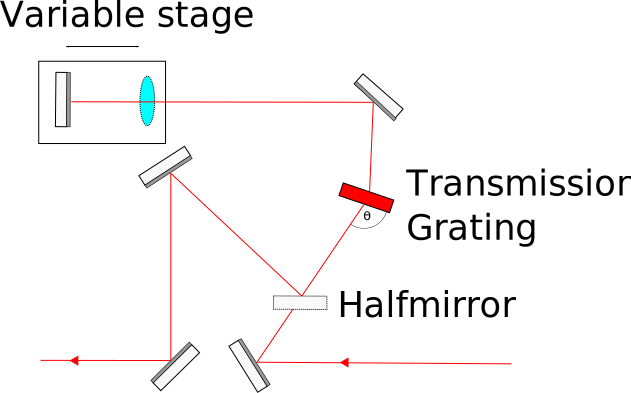
\includegraphics[width=0.7\linewidth]{figures/chirp/pulse-expander}
	\caption{}
	\label{fig:pulse-expander}
\end{figure}



\section{Adiabatic rapid passage}
One way to inverse the \ac{QD} from the ground state to the biexciton state is by exciting it with a transform-limited laser pulse of constant center frequency, which is equals to half of the ground state biexciton transition frequency.
However, in order to ensure the inversion precise control of the field intensity is required~\cite{glassl_biexciton_2013}.
Adiabatic rapid passage \acused{ARP} (\acs{ARP}) with frequency chirped is an alternative to this Rabi-flopping scheme.
Basically, the goal is to adiabatic state from ground state to biexciton state without energy-level crossing~\cite{hui_proposal_2008}.
Schemes which provide that, are also stable with respect to intensity changes of the laser field.

In order to calculate the final biexciton occupation, \textcite{glassl_biexciton_2013} assumed linearly-chirped Gaussian laser pulse as discussed in section~\ref{sec:chirp}.
The simulation results are visible in figure~\ref{fig:biexciton-occupation}.
\begin{figure}[H]
	\centering
	\includegraphics[width=\linewidth]{figures/chirp/biexciton-occupation}
	\caption{Final biexciton occupation after chirped Gaussian pulse of pulse duration $\tau_0 = \SI{2}{\pico \second}$.
		It is plotted vertically as a function of the original pulse area $A$ and vertically as a function of the chirp $\alpha$ for biexciton binding energies of (a) $\Delta=0$, (b) 1, and (c) \SI{3}{\milli \electronvolt}~\cite{glassl_biexciton_2013}.}
	\label{fig:biexciton-occupation}
\end{figure}
The central frequency is chosen so that for $\alpha=0$ it resonates to ground state biexction transition, which is sketched in figure~\ref{fig:biexciton-occupation}.
For $\alpha=0$ Rabi oscillations are visible and its period depends strongly on the biexciton binding energy $\Delta$.
However, for $\alpha \gg 0$ biexciton preparation becomes insensitive to small variations to the pulse area $A$ as long it exceeds a certain threshold.
In the case of $\alpha < 0$ this fails for moderate values of $\Delta$ as can be seen in figure~\ref{fig:biexciton-occupation}(b).


\section{Simulation}

\begin{figure}[H]
	\centering
	\includegraphics[width=\linewidth]{figures/chirp/plots/chirped_laser_pulse}
	\caption{Electric field $E$ of Gaussian laser pulse of pulse duration $\tau_0=\SI{0.5}{\pico \second}$ for chirp of (a) $\alpha = \SI{0}{\pico \second \squared}$ and (b) $\alpha = \SI{0.5}{\pico \second \squared}$}
	\label{fig:chirpedlaserpulse}
\end{figure}

\begin{figure}[H]
	\centering
	\includegraphics[width=\linewidth]{figures/chirp/plots/I_M_gauss_chirp_without_slit_without_MOSAIC}
	\caption{Intensity of IAC of a Gaussian laser pulse of pulse duration $\tau_0=\SI{0.5}{\pico \second}$ with applied MOSAIC filter for chirp of (a) $\alpha = \SI{0}{\pico \second \squared}$ and (b) $\alpha = \SI{0.5}{\pico \second \squared}$}
	\label{fig:imgausschirpwithoutslitwithoutmosaic}
\end{figure}


\begin{figure}[H]
	\centering
	\includegraphics[width=\linewidth]{figures/chirp/plots/mosaic_chirped_laser_pulse}
	\caption{Intensity of IAC of a Gaussian laser pulse of pulse duration $\tau_0=\SI{0.5}{\pico \second}$ with applied MOSAIC filter for chirp of (a) $\alpha = \SI{0}{\pico \second \squared}$ and (b) $\alpha = \SI{0.5}{\pico \second \squared}$}
	\label{fig:mosaicchirpedlaserpulse}
\end{figure}

\begin{figure}[H]
	\centering
	\includegraphics[width=\linewidth]{figures/chirp/plots/mosaic_chirped_laser_pulse_find_envelope}
	\caption{Intensity of IAC of a Gaussian laser pulse of pulse duration $\tau_0=\SI{0.5}{\pico \second}$ with applied MOSAIC filter for chirp of (a) $\alpha = \SI{0}{\pico \second \squared}$ and (b) $\alpha = \SI{0.5}{\pico \second \squared}$.
	The orange dots are results of a numerical peak finder algorithm, executed in order to find local minima.}
	\label{fig:mosaicchirpedlaserpulsefindenvelope}
\end{figure}

See \textcite{hirayama_real-time_2002}

The lower bound (minima envelope) of the MOSAIC trace is therefore given by

\begin{equation}
S^{min}_{MOSAIC}(\tau)= 1 + 2 \cdot g(\tau) - 2 \cdot [g_s^2(\tau)+g_c^2(\tau)]^{1/2}
\end{equation}

with 

\begin{align}
g(\tau)&=\int f(t)f(t+\tau)dt\\
g_s(\tau)&=\int f(t)f(t+\tau)sin(2\Delta\phi)dt\\
g_c(\tau)&=\int f(t)f(t+\tau)cos(2\Delta\phi)dt
\end{align}


\begin{figure}[H]
	\centering
	\includegraphics[width=\linewidth]{figures/chirp/plots/mosaic_chirped_laser_pulse_fit_envelope}
	\caption{Intensity of IAC of a Gaussian laser pulse of pulse duration $\tau_0=\SI{0.5}{\pico \second}$ with applied MOSAIC filter for chirp of (a) $\alpha = \SI{0}{\pico \second \squared}$ and (b) $\alpha = \SI{0.5}{\pico \second \squared}$.
	The orange line is a fit for the lower envelope of the MOSAIC signal in order to obtain $\alpha$.}
	\label{fig:mosaicchirpedlaserpulsefitenvelope}
\end{figure}




\section{Measurements and discussion}

\begin{figure}[H]
	\centering
	\includegraphics[width=\linewidth]{figures/chirp/plots/measured_chirped_laser_pulse_before_MOSAIC}
	\caption{Measured IAC of Ti:Sa Laser without (a) and with (b) pulse expander before the autocorrelator.}
	\label{fig:measuredchirpedlaserpulsebeforemosaic}
\end{figure}

\begin{figure}[H]
	\centering
	\includegraphics[width=\linewidth]{figures/chirp/plots/measured_chirped_laser_pulse_after_MOSAIC}
	\caption{Measured IAC of Ti:Sa Laser with applied MOSAIC filter without (a) and with (b) pulse expander before the autocorrelator.}
	\label{fig:measuredchirpedlaserpulseaftermosaic}
\end{figure}


